\section{LibreCAD v3 Kernel Development}
This is the CAD Kernel I have devloped during my 6 week training project. Iwas hired by Google for 3 months and paid a stipend of Rs. 300000 during the work. This CAD kernel is developed for the opensource CAD organisation LibreCAD under the supervision of BRL-CAD. 
\begin{figure}[h]
\begin{center}
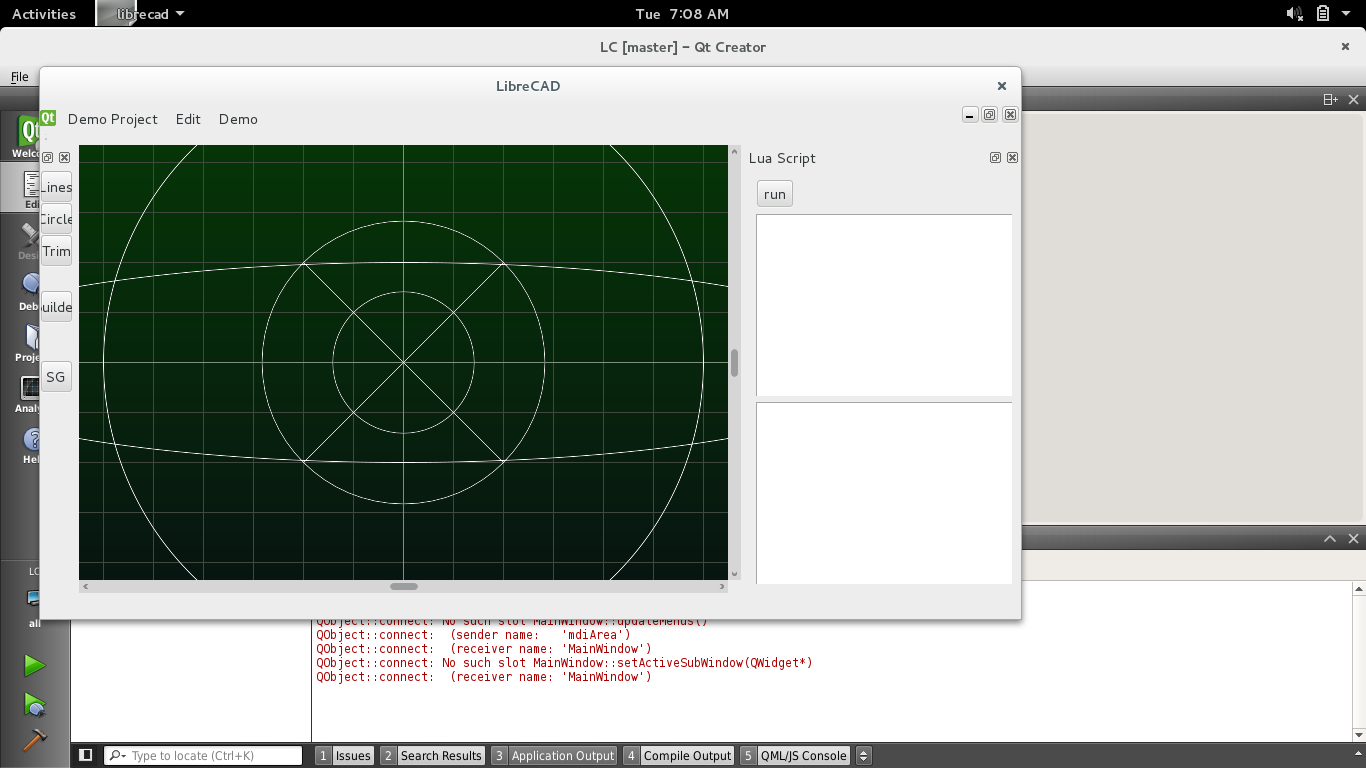
\includegraphics[scale=0.3]{images/cad/simplerun.png}
\caption{v3- The advanced 2D kernel}
\end{center}
\end{figure}

It has the following features:
\begin{itemize}
\item New
\item Undo
\item Redo
\item Add Random Circle
\item Add Random Arc
\item Add Random Lines
\item Clear Undo Stack
\end{itemize}

The idea of LibreCAD v3 Kernel Development was to build a stable kernel for the improvement of CAD and Opensource CAD. LibreCAD 3 has been divided into 3 modules.

\begin{itemize}
\item Kernel
\item Viewer
\item UI
\end{itemize}

Though the code is still in development, variations may apply. There is an additional module for scripting. Users can develop their on modules in their preferred langauge may it be python, lua, ruby.
We preferred lua since it was lightweight and simple.
The UI part of LibreCADv3 is to be rewritten hence it is disabled at the moment. Figures can be drawn using the lua script coding.

\begin{figure}[h]
\begin{center}
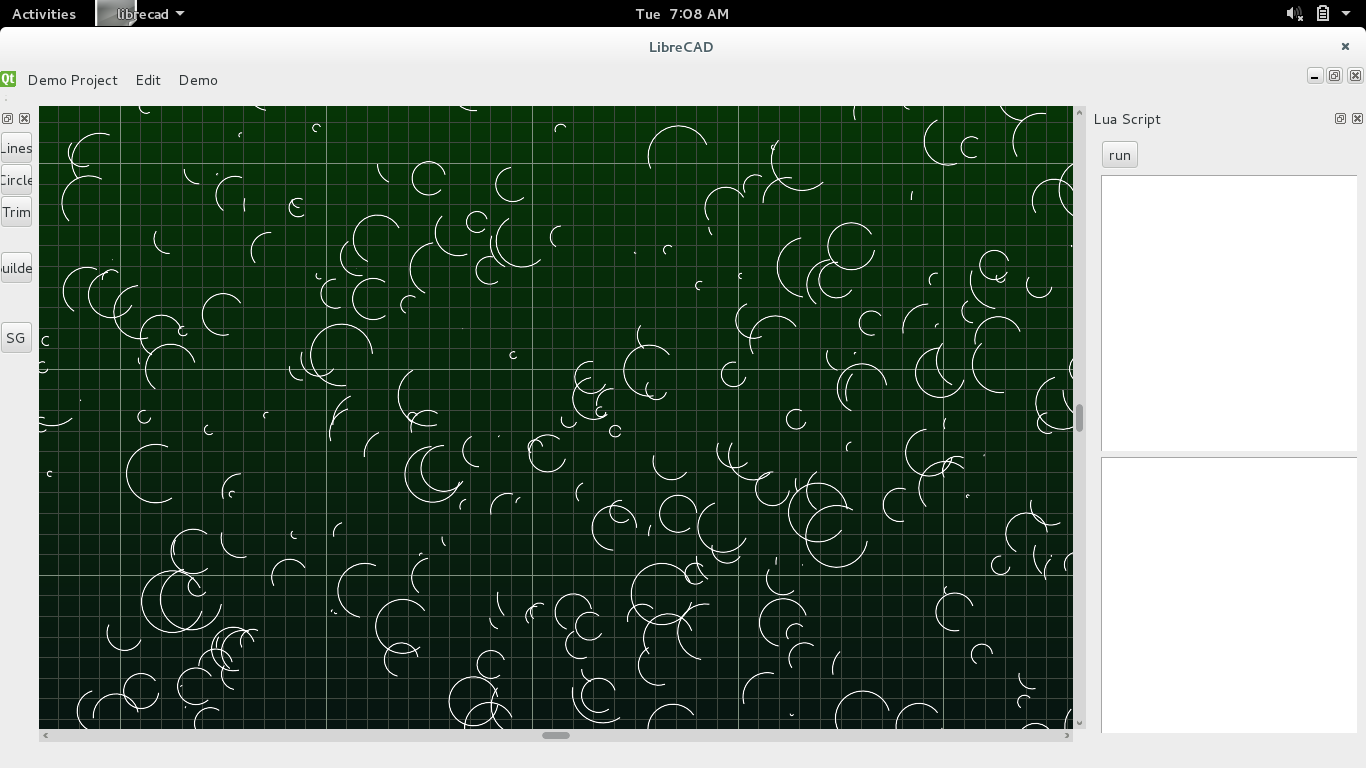
\includegraphics[scale=0.3]{images/cad/randomarc.png}
\caption{ Random arcs generated while testing. }
\end{center}
\end{figure}
\begin{figure}[h]
\begin{center}
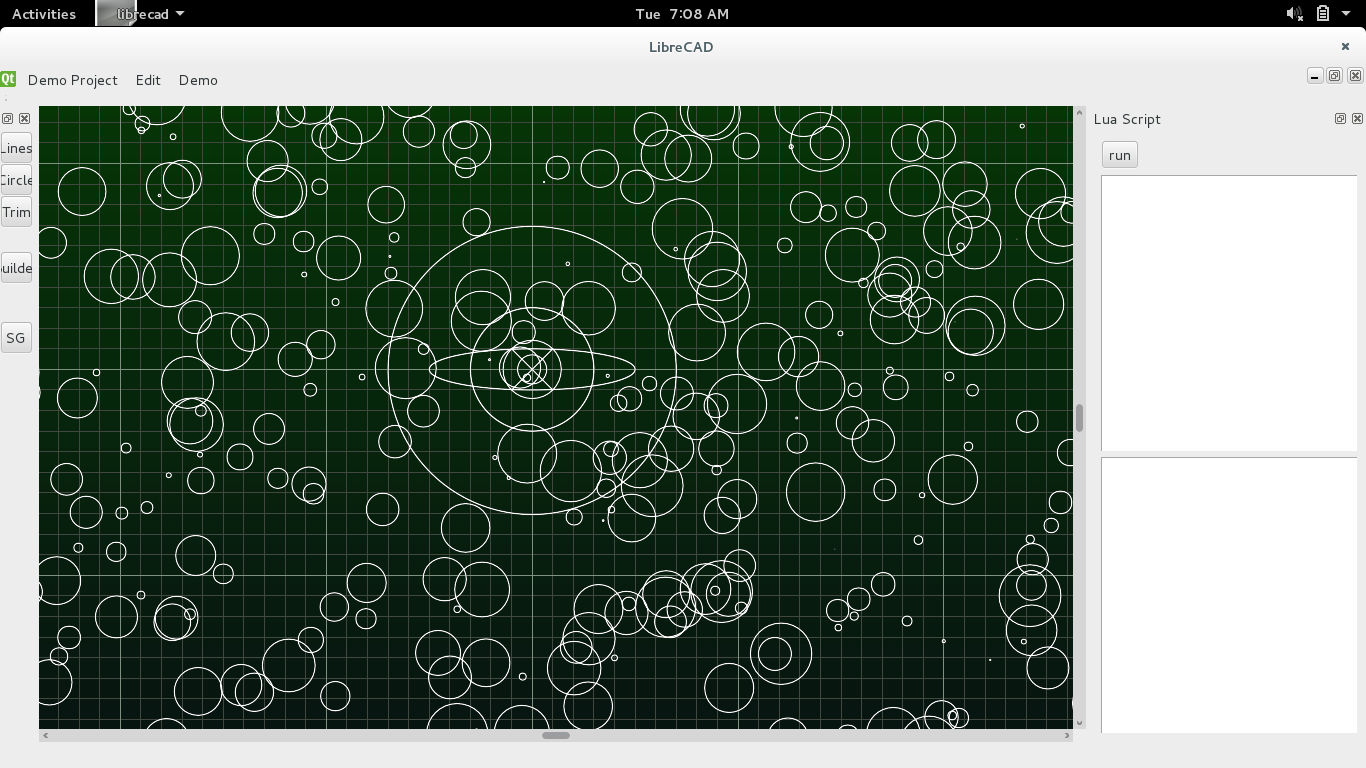
\includegraphics[scale=0.3]{images/cad/randomcircle.png}
\caption{ Random Circles generated during testing. }
\end{center}
\end{figure}
\begin{figure}[h]
\begin{center}
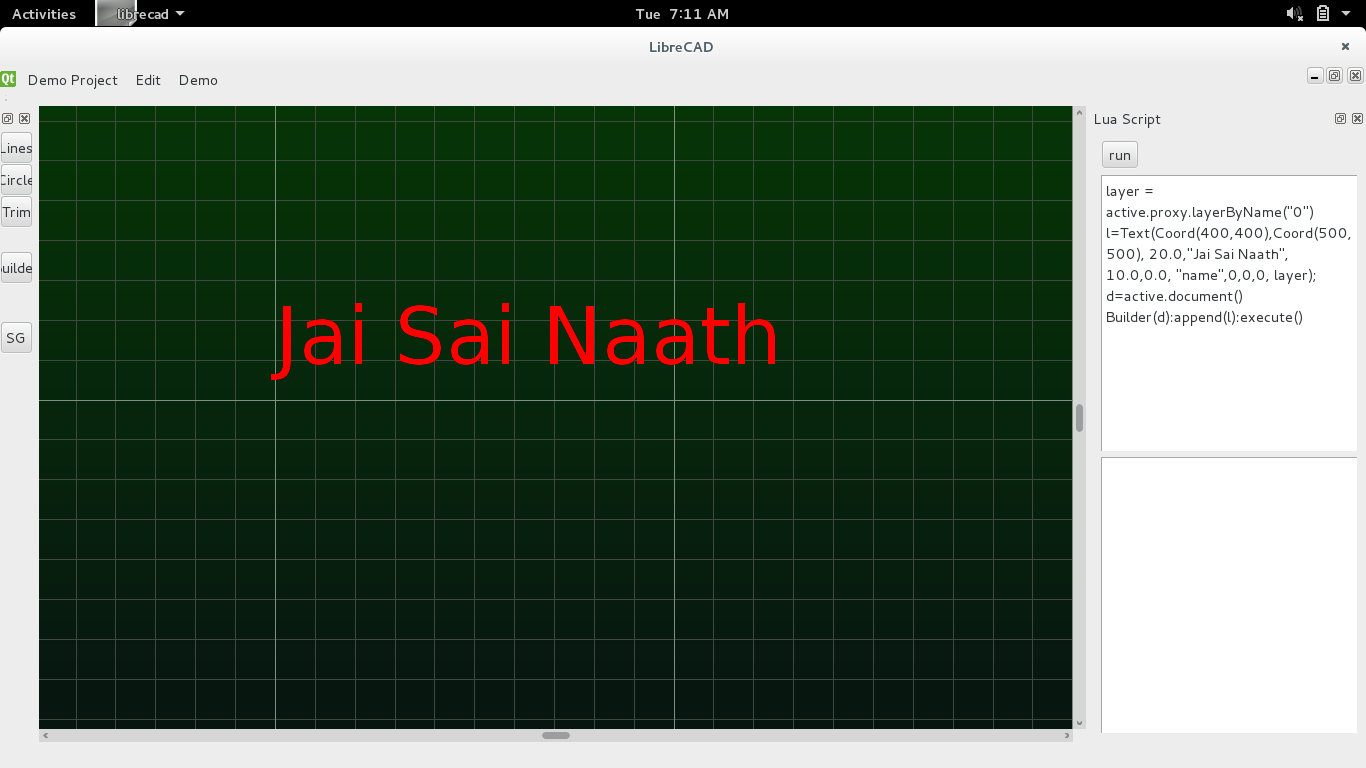
\includegraphics[scale=0.3]{images/cad/text.png}
\caption{ The Text entity implementation. }
\end{center}
\end{figure}
\begin{figure}[h]
\begin{center}
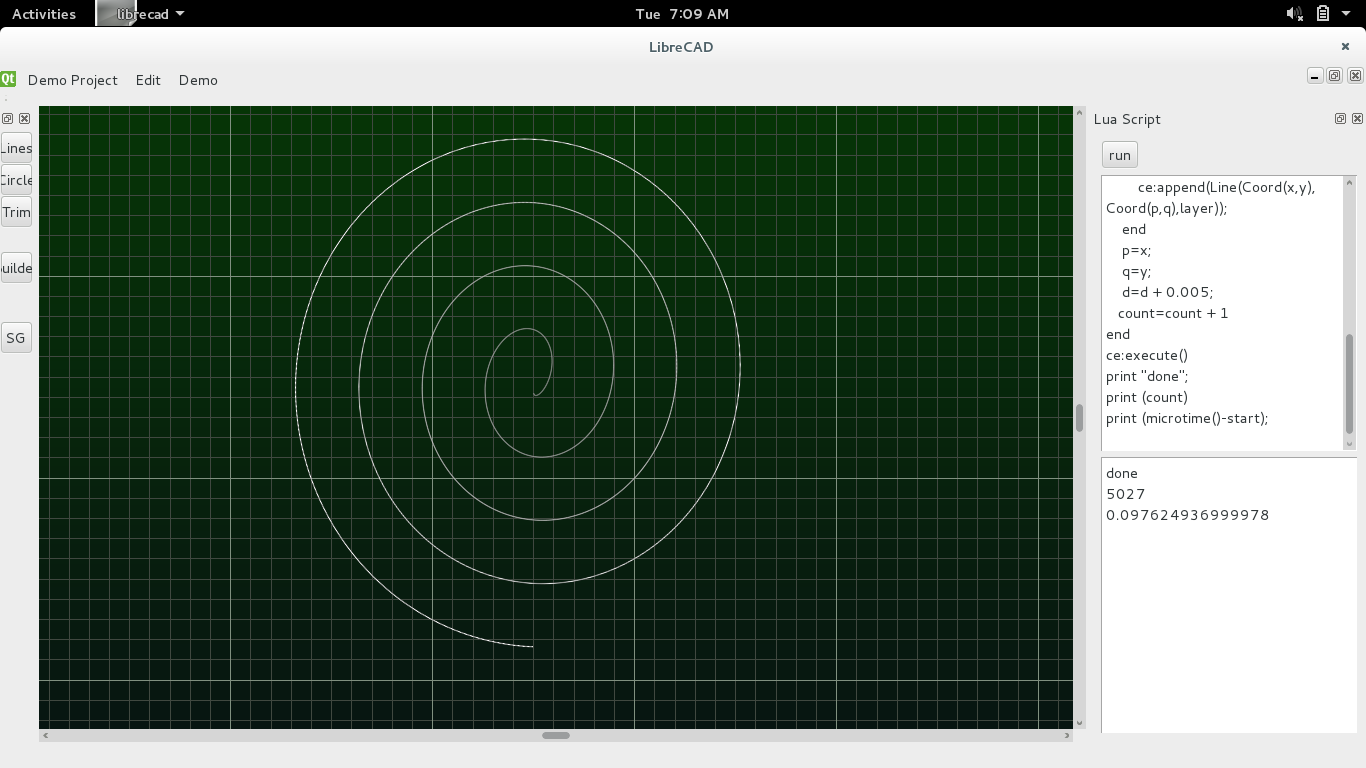
\includegraphics[scale=0.3]{images/cad/spiral.png}
\caption{ Spiral Drawn with the scripting module of LibreCAD 3 using Lua language. }
\end{center}
\end{figure}
\begin{figure}[h]
\begin{center}
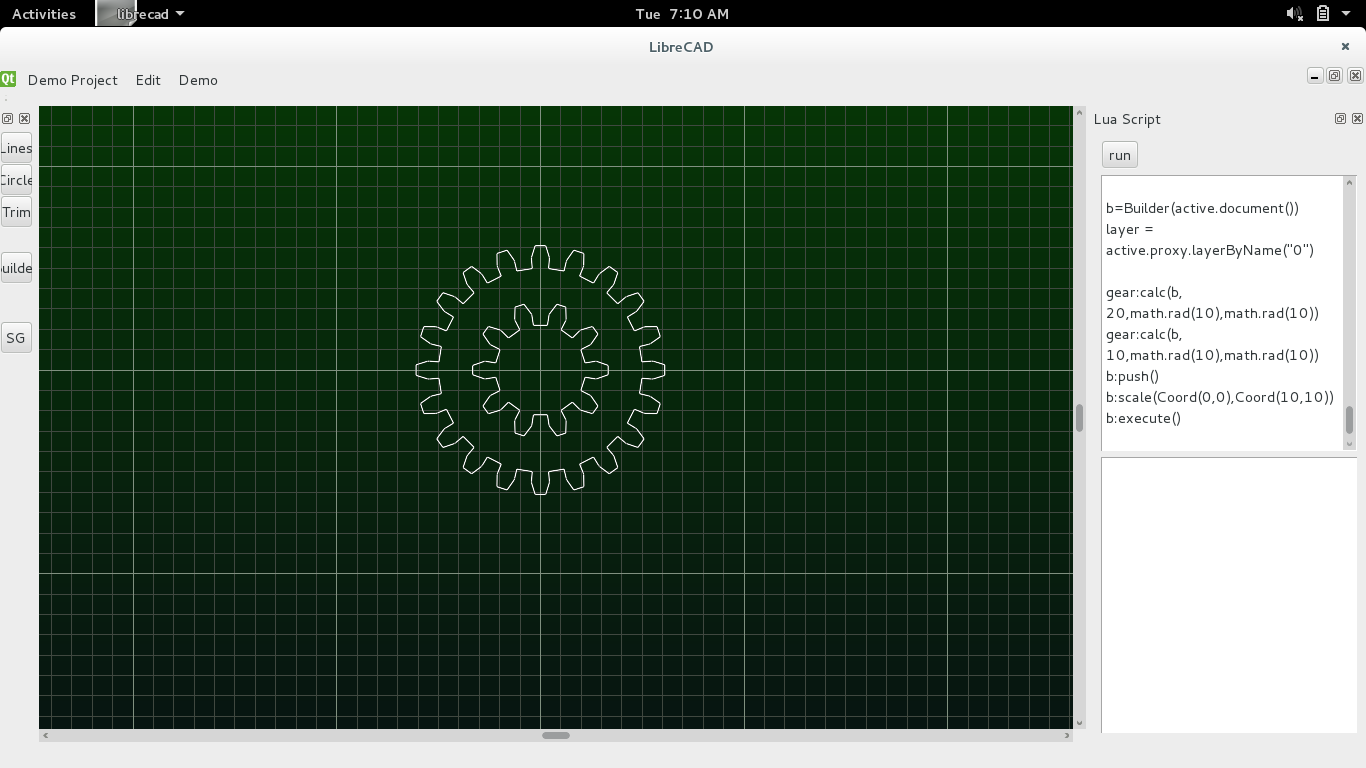
\includegraphics[scale=0.3]{images/cad/gear.png}
\caption{ Gear module drawn using LibreCAD 3 scripting.}
\end{center}
\end{figure}
\begin{figure}[h]
\begin{center}
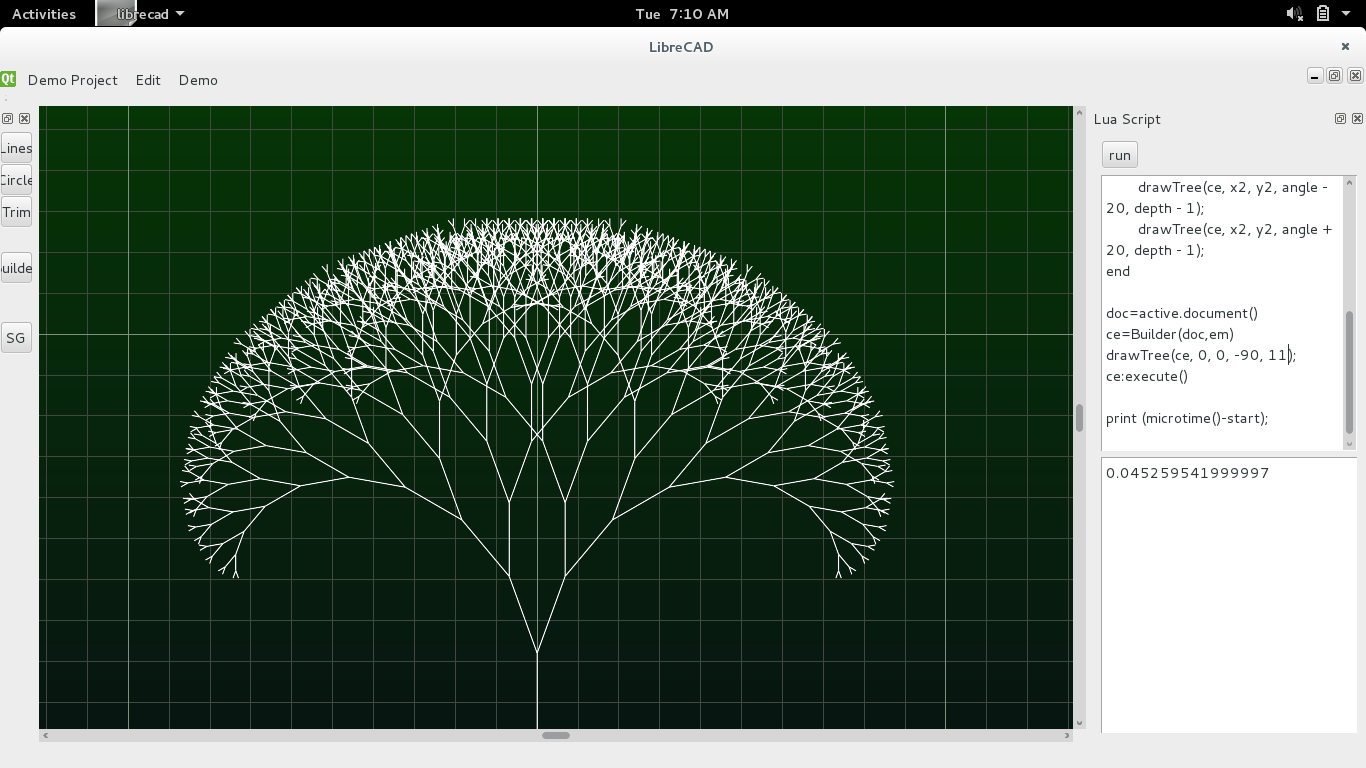
\includegraphics[scale=0.3]{images/cad/fractaltree.png}
\caption{ fractaltree drawn using LibreCAD 3 scripting. }
\end{center}
\end{figure}

\subsection{Installation Guide}
To install v3, you need to clone it from github.
\begin{itemize}
\item Go to terminal and type\\\\
\textit{git clone http://www.github.com/gaganjyot/LibreCAD3.git}
\item Now go to the directory vEdit by using: \\\\
\textit{cd LibreCAD3}
\item Now running cmake command: \\\\
\textit{cmake vEdit.pro}
\item Now MakeFile will be generated. After that run make: \\\\
\textit{make}
\item An executable file will be generated. Execute it using: \\\\
\textit{./lcUI/librecad}
\end{itemize}
